\documentclass[a4paper,11pt]{article}
\usepackage{gensymb}
\usepackage{blindtext}
\usepackage{titlesec}
\usepackage[english]{babel}
\usepackage{amsthm}
\usepackage{amsmath}
\usepackage{amssymb}
\usepackage{tikz, pgfplots}
\usepackage{titlesec}
\usepackage{lipsum}
\usepackage{xcolor} 
\usepackage{float}
\usepackage{hyperref}
\hypersetup{hidelinks}
\usepackage{xparse}

\ExplSyntaxOn
\NewDocumentCommand{\cycle}{ O{\;} m }
 {
  (
  \alec_cycle:nn { #1 } { #2 }
  )
 }

\seq_new:N \l_alec_cycle_seq
\cs_new_protected:Npn \alec_cycle:nn #1 #2
 {
  \seq_set_split:Nnn \l_alec_cycle_seq { , } { #2 }
  \seq_use:Nn \l_alec_cycle_seq { #1 }
 }
\ExplSyntaxOff

\numberwithin{equation}{section}
\def\llbracket{[\![}
\def\rrbracket{]\!]}

\title{Pólya's Enumeration Theorem}
\date{April 2025}
\author{Damilare Fagbile}
\renewcommand{\thesection}{\arabic{section}}

\makeatletter
\renewcommand{\maketitle}{%
    \begin{center}
        {\LARGE  \@title} \\[2ex]  
        {\large \@author} \\[1ex]
        {\large \@date}
    \end{center}
}

\newenvironment{chapquote}[2][2em]
  {\setlength{\@tempdima}{#1}%
   \def\chapquote@author{#2}%
   \parshape 1 \@tempdima \dimexpr\textwidth-2\@tempdima\relax%
   \itshape}
  {\par\normalfont\hfill--\ \chapquote@author\hspace*{\@tempdima}\par\bigskip}


\makeatother

\titleformat{\subsection}[runin]% runin puts it in the same paragraph
       {\normalfont\bfseries}% formatting commands to apply to the whole heading
       {\thesubsection}% the label and number
       {0.5em}% space between label/number and subsection title
       {}% formatting commands applied just to the subsection title
       [.]% punctuation or other commands following subsection title

\titleformat{\subsubsection}[runin]% runin puts it in the same paragraph
       {\normalfont\bfseries}% formatting commands to apply to the whole heading
       {\thesubsubsection}% the label and number
       {0.5em}% space between label/number and subsection title
       {}% formatting commands applied just to the subsection title
       [.]% punctuation or other commands following subsection title




\begin{document}
    \nocite{*}
    
    \maketitle

    \section{Introduction}
    \label{sec: intro}

    The main result in this essay is most easily understood in terms of colourings of finite objects, so consider the following example. How many ways can one colour the beads in the following arrangement using two colours, say blue and brown? 
    
    \begin{figure}[H]
    \centering
        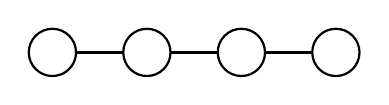
\begin{tikzpicture}
            % Define bead radius
            \def\r{0.3}
            % Draw the string behind the beads, only between them
            \draw[thick] (0+\r,0) -- (1.2-\r,0);
            \draw[thick] (1.2+\r,0) -- (2.4-\r,0);
            \draw[thick] (2.4+\r,0) -- (3.6-\r,0);
            % Draw the circles (beads)
            \foreach \x in {0,1.2,2.4,3.6} {
                \draw[thick,fill=white] (\x,0) circle(\r);
            }
        \end{tikzpicture}
        \caption{String of four beads we wish to colour.}
        \label{fig: 1}
    \end{figure}

    \begin{figure}[H]
        \centering
        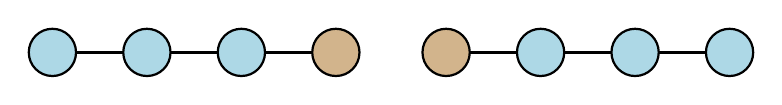
\begin{tikzpicture}
        % Define bead radius
        \def\r{0.3}
        % Define colours
        \definecolor{beadblue}{RGB}{173,216,230} % Light Steel Blue
        \definecolor{beadbrown}{RGB}{210,180,140} % Tan
        % Draw the string 
        \draw[thick] (0+\r,0) -- (1.2-\r,0);
        \draw[thick] (1.2+\r,0) -- (2.4-\r,0);
        \draw[thick] (2.4+\r,0) -- (3.6-\r,0);
        % Draw the circles (beads) with colours
        \fill[beadblue] (0,0) circle(\r);
        \fill[beadblue] (1.2,0) circle(\r);
        \fill[beadblue] (2.4,0) circle(\r);
        \fill[beadbrown] (3.6,0) circle(\r);
        \foreach \x in {0,1.2,2.4,3.6} {
            \draw[thick] (\x,0) circle(\r);
        }
        
        % Draw the second row of beads to the right
        \begin{scope}[xshift=5cm]
            % Draw the string 
            \draw[thick] (0+\r,0) -- (1.2-\r,0);
            \draw[thick] (1.2+\r,0) -- (2.4-\r,0);
            \draw[thick] (2.4+\r,0) -- (3.6-\r,0);
            % Draw the circles (beads) with colours
            \fill[beadbrown] (0,0) circle(\r);
            \fill[beadblue] (1.2,0) circle(\r);
            \fill[beadblue] (2.4,0) circle(\r);
            \fill[beadblue] (3.6,0) circle(\r);
            \foreach \x in {0,1.2,2.4,3.6} {
                \draw[thick] (\x,0) circle(\r);
            }
        \end{scope}
        \end{tikzpicture}
        \caption{The `same' colouring?}
        \label{fig: 2}
    \end{figure}

   Since each bead is coloured independently in one of two ways, the total number of possible colourings is $2^4$, applying the so-called product rule for counting. In particular, there $\binom{4}{k}$ colourings with exactly $k$ blue beads, where $\binom{4}{k}$ denotes a binomial coefficient. These subsets partition the set of all colourings, which yields the following identity \[\binom{4}{1} + \binom{4}{2} + \binom{4}{3} + \binom{4}{4} = 2^4,\] an instance of a \textit{double--counting} argument. 
   
   \subsection{Generating Functions} The same identity, however, can be derived algebraically by applying the binomial theorem
   \begin{equation}
        \label{eq: binomial_theorem}
        \sum\limits_{n=0}^{4} \binom{4}{n} x^{n} = (1+x)^{4} 
    \end{equation}
    and substituting \(x=1\). The sum \(\sum_{n=0}^{4} {4 \choose n} x^{n}\) is known as a \textit{generating function} for the sequence $\left({4 \choose n}\right)_{n=1}^{4}$. Generating functions -- essentially polynomials or formal power series -- are a powerful tool in enumerative combinatorics, as they allow us to apply methods of algebra and complex analysis (when they converge) to enumeration (i.e., counting). For example, they may allow one to derive an explicit formula for their sequence: applying the formal differential operator $(d/{dx})^k$ to both sides of \eqref{eq: binomial_theorem} and substituting $x=0$ gives $k! \binom{4}{k} = {4!}/{(4-k)!}$, rediscovering the well-known formula for binomial coefficients. \smallskip 
    
    Even when one cannot find a pleasant explicit formula for a sequence, their generating functions may allow us to find their asymptotic distribution (like in the Prime Number Theorem or the Hardy-Ramanujan partition function asymptotics) and other deeper properties (see \cite[p.~2]{wilf2006generatingfunctionology} and \cite[Section VIII.6.]{flajoletAnalyticCombinatorics2013}). \smallskip
    
    That said, we still seek combinatorial proofs -- those involving double counting or bijections -- as they are more explanatory.  Although generating functions proofs are not combinatorial, they can often suggest the equivalence of two sets in a way that leads to a combinatorial understanding, as we shall see in some examples. After all, if two sets have the same cardinality, we should be able to construct a bijection between them. 
    
    \subsection{The General Setup} Now suppose we can rotate the beads string in Figure \ref{fig: 1} by $180 \degree$. Then two colourings that differ only by a \(180^\circ\) rotation (as shown in Figure \ref{fig: 2}, for example) are considered equivalent. How many colourings are there up to $180^\circ$ rotation? In our original count, the colourings that are not fixed by \(180^\circ\) are double-counted while those that are fixed by \(180^\circ\) are counted once. The colourings that are fixed by \(180^\circ\) rotation are exactly those where the first and last beads are the same colour as well as the second and third beads, so they are uniquely determined by our choice of the first two colours, which yields \(2^2\) such colourings. Therefore, the total number of colourings up to a \(180^\circ\) rotation is given by\begin{align*}
        &\#\{ \text{colourings} \mid  \text{fixed by $180 \degree$ rotation} \}   \\
        &+ \frac{1}{2} \# \{ \text{colourings} \mid  \text{not fixed by $180 \degree$ rotation} \}   
    \end{align*} Since the fixed and non-fixed colourings together account for all colourings, this expression can be rewritten as \begin{align}
         &\frac{1}{2} \left ( \#\{ \text{colourings} \mid  \text{fixed by $180 \degree$ rotation} \}+ \# \{ \text{colourings}  \} \right) \label{eq: burnsides_lemma_example} \\
        &= \frac{1}{2} (2^2 + 2^4)=10. \nonumber 
    \end{align}
    We can continue applying \eqref{eq: burnsides_lemma_example} to find that there are exactly $1, 2,$ and $4$ inequivalent colourings using $0, 1,$ and $2$ blue beads respectively. Moreover, the number of inequivalent colourings using $k$ blue beads is the same as the number of colourings using $4-k$ blue beads, since there is a natural bijection between the sets counted: swapping the colours blue and brown. We summarise these counts with the following bivariate generating function, where the coefficient of $c_{1}^k c_{2}^{l}$ is the number of inequivalent colourings with $k$ blue beads and $l$ brown beads 
    \begin{equation} 
    \label{eq: example-pattern_inventory}
        c_{1}^4 + 2c_{1}^3c_{2} + 4c_{1}^{2}c_{2}^{2} + 2c_{1}c_{2}^3 + c_{2}^4. 
    \end{equation}\smallskip
    
    More generally, throughout this essay, we will have have: a finite set $D$, which we think of as the object we wish to colour; an at most countable set $C= \{c_1, c_2, \dots \}$, which we think of as our palette of colours; and a group $G$ of permutations of $D$. A function $f:D\to C$ then represents a colouring of $D$; hence our choice of letters -- $D$ for domain and $C$ for codomain. Since the product rule asserts that $\# \{f:C \to D\} = (\# C)^{\#D}$, we use $C^D$ to denote\footnote{The reader should be familiar with the use of this notation for the Cartesian power $A^n$ which can be identified as the set of all functions $f:\{1,2,...,n\} \to A$.} $\{f:D\to C\}$, the set of all functions from $D$ to $C$. Two colourings $f_1,f_2\in C^D$ are what Stanley \cite{stanley2013} calls \textit{$G$-equivalent} if $f_1$ can be factored (need not be unique) as $f_2 \circ g$ for some $g \in G$.  \smallskip
    
    In our string-of-four-beads example, if we label the beads in Figure \ref{fig: 1} with $1$ through $4$ from left to right then $D= \{1,2,3,4\}$ and $C=\{c_1, c_2\}$ where $c_1$ and $c_2$ represent blue and brown respectively. Our permutation group is the group generated by the permutation $\pi= \cycle[,]{1,4} \cycle[,]{2,3}$ which represents $180^\circ$ rotation:
    \begin{equation}
        \label{eq: example-group}
        G = \left \{ \cycle{1} \cycle{2} \cycle{3} \cycle{4} , \; \cycle[,]{1,4} \cycle[,]{2, 3} \right \}.
    \end{equation}
    The colourings on the left and right of Figure \ref{fig: 2} are represented by the functions $f_1,f_2\in C^D$ defined by 
    \begin{align*}
        f_1: \{1,2,3\} \mapsto c_1,\ 4 \mapsto c_2, \\
	    f_2: \{4,2,3\} \mapsto c_1,\ 1 \mapsto c_2.
    \end{align*}Hence, these colourings are equivalent because $f_1 = f_2 \circ \pi$.  \smallskip
    
    It takes a routine check to verify that $G$--equivalence satisfies the conditions of reflexivity, symmetry and transitivity and is thus an equivalence relation. However, more conceptually, this follows from the fact that \(G\)-equivalence corresponds to membership in the same orbit under the \textit{composition action} of \(G\) on \(C^D\). Composition indeed defines a right group action as it satisfies the identity and compatibility axioms: \(f\circ \text{Id}_D = f\) and \((f\circ g_1)\circ g_2 = f\circ (g_1\circ g_2) \) for all $f\in C^D$ and $g_1, g_2 \in G$. \smallskip
 
    Our motivation is to be able to answer the same questions as before. How many inequivalent colourings are there? How many inequivalent colourings use each colour a specified number of times? In particular, regarding the $c_j$ as indeterminates (formal variables), we seek a formula -- reminiscent of the binomial theorem in \eqref{eq: binomial_theorem} -- for the multivariate generating function of the numbers of inequivalent colourings:
    \begin{equation}
        \label{eq: pattern_inventory}
        \sum_{i_1 + i_2 + \cdots = n} \#(S_{i_1, i_2, ...} / G)  c_1^{i_1}c_{2}^{i_2}\cdots \tag{1.5}
    \end{equation}where $S_{i_1, i_2, \dots}\subset C^D$ is the the subset of colourings where the colour $c_{j}$ is used $i_j$ times and \(S_{i_1, i_2, \dots}/G\) denotes the orbit space in \(S_{i_1, i_2, \dots}\) under the composition action of \(G\) so that $\#(S_{i_1, i_2, \dots}/G)$ is the number of inequivalent colourings where colour $c_j$ is used $i_j$ times. \smallskip
    
    The main goal of this essay is to present a modern exposition of Pólya's enumeration theorem, which provides a closed formula for this generating function. In his original paper \cite{Polya1937}, Pólya explored applications of his formula to enumerating non--isomorphic graphs, trees, chemical compounds and their asymptotic analysis -- none of which are covered here. Many, many more miscellaneous applications were discussed by Read in his English translation of Pólya's paper \cite[p.~134]{PolyaTranslation1987}. Nonetheless, the author considers several elementary examples that aid understanding of Pólya's formula and its far-reaching applications.

    \section{Burnside's Lemma} 

    \begin{chapquote}{Tim Gowers \cite{GroupActionsII2011}}
    ``The content of the orbit-stabilizer theorem is basically that if a group $G$ acts on a set $X$, then once you know how many ways there are of sending an element $x$ of $X$ to itself, you also know how many ways there are of sending it to any other element in its orbit.''
    \end{chapquote}  

    In this section, we generalise our setup by considering a finite abstract group $G$, which need not be a group of permutations, acting on a finite set $X$, which need not be a set of functions. As in \eqref{eq: burnsides_lemma_example}, we'll see that we can always reduce enumerating the set of orbits $X/G$ to enumerating $X^{g}$, the subset of $X$ fixed by $g$, for each $g \in G$. \smallskip

    A fixed point is a pair $(g,x)$ such that $g*x = x$. Counting such pairs ``vertically", then ``horizontally", yields the following 
    \begin{equation}
        \sum_{x\in X} \# \text{Stab}_G(x)  = \sum_{g\in G} \# X^g,   \label{eq: ver_hor}\tag{1.1}
    \end{equation} where $\text{Stab}_G(x)$ denotes the stabilizer of $x$, the subset of $G$ that fixes $x$, $x\in X$. For an orbit $O\in X/G$, the orbit--stabilizer theorem asserts that $\sum_{x\in O} \# \text{Stab}_G(x) = \#G$ (or equivalently, $\#\text{Stab}_G(x)\cdot \#O = \#G$, for any $x\in O$, since the $\# \text{Stab}_G(x)$ are the same) which follows from the existence of a natural bijection between $O$ and $G/\text{Stab}_G(x)$, for any $x\in O$.  \smallskip
    
    Furthermore, we can rewrite the left-hand side of \eqref{eq: ver_hor} as \break $\sum_{O \in X/G} \sum_{x\in O} \# \text{Stab}(x)$, since $X/G$ forms a partition $X$, which immediately gives the following result known popularly as \textit{Burnside's lemma}, or the \textit{Cauchy-Frobenius lemma}.
    \subsection{Lemma} \label{lemma: burnside's} Let $G$ be a finite group acting on a finite set $X$ and let $X/G$ denote the set of orbits in $X$ under this action. Then \begin{equation*}
        \# (X \text{/} G) = \frac{1}{\# G} \sum_{g\in G} \# X^{g}, \label{eq: ch2} \tag{1.2}
    \end{equation*}  where $X^{g}=\{ x\in X \mid g*x=x \}$, the subset of $X$ fixed by $g$. That is, the number of orbits is the average number of fixed points over the elements of $G$.\footnote{The number of fixed points for $g\in G$ is exactly the trace of its linear permutation representation, an example of a character \cite{wiki:Permutation_representation}. Such averaging arguments appear frequently in character theory.} \medskip

    Burnside stated and proved Lemma \ref{lemma: burnside's} in \cite[Sects. 118–119]{Burnside1911},  but it was
    first stated and proved by Frobenius, who, in turn, credited Cauchy with proving the lemma in the special case of a transitive group action (i.e., a single orbit). As a result, many authors now refer to this result as the Cauchy–Frobenius lemma instead. See \cite{Neumann1979} for a more detailed historical account.

    
    \subsection{Example} 
    \label{eg: ch2}How many subsets of \(\llbracket 2025 \rrbracket = \{1, 2, \dots, 2025\}\) have the property that their sum, i.e. the sum of their elements, is divisible by 5? \smallskip
    
    Titu and Zuming \cite[p.~58]{andreescu2002102} show that the answer is $\frac{1}{5}(2^{2025} + 4 \cdot 2^{405})$ using a generating function proof that can be summarised as follows. Let $a_n$ be the coefficient of $x^n$ in the expansion of following polynomial \[f(x) = (1+x)(1+x^2) \cdots (1+x^{2025}).\]Then $a_n$ counts the number of subsets of \(\llbracket 2025 \rrbracket \) that sum to \(n\) since there is a bijection between subsets of \( \llbracket 2025 \rrbracket\) and monomials appearing in the expansion of \(f(x)\), where a subset \(S = \{s_1, s_2, \dots, s_k\}\) corresponds to the monomial \( x^{s_1}x^{s_2} \cdots x^{s_k} = x^{s_1 + s_2 + \dots + s_k} \). Hence, we are looking for the sum of coefficients $a_0 + a_5 + a_{10}+\cdots$ which can be found using a `root of unity filter'. Let \(\zeta = \exp(2\pi i/5) \) be a $5$th root of unity. Then $\zeta^5=1$ and $1+\zeta+\zeta^2+\zeta^3+\zeta^4 = 0$ which yield $a_0+ a_5+ a_{10}+\cdots = \frac{1}{5}\sum_{j=0}^{4} f(\zeta^j)$. This proves our claim (see the reference for details). \medskip
    
    However, the given formula suggests an alternative approach involving Burnside’s lemma. We now present a double--counting argument that considers the orbits in \(2^{\llbracket 2025 \rrbracket} \), the set of subsets of $\llbracket 2025 \rrbracket$, under the action of a suitable group of order $5$. \medskip

   Consider the following permutation of \(\llbracket 2025 \rrbracket\) 
    \[\pi = \cycle[,]{1,2,3,4,5} \cycle[,]{6,7,8,9,10} \cdots \cycle[,]{2020, 2021, 2022, 2023, 2024, 2025}.\]
    
    Let $\langle \pi \rangle = \{ \text{Id}, \pi, \pi^{2}, \pi^{3}, \pi^{4} \}$ be the group generated by $\pi$. Naturally, \(\langle \pi \rangle\) acts on \( 2^{\llbracket 2025 \rrbracket} \) by applying $\pi$ to each element of a subset $S$: \break $\pi*S=\{ \pi (s)\mid s\in S \}$, $S\in 2^{\llbracket 2025 \rrbracket}$. For example, the orbit of $\{ 1\}$ under this action is given by $\left\{\begin{array}{c}\{1\}, \{2\}, \{3\}, \{4\}, \{5\}\end{array}\right\}$. \medskip
    
    Observe that $S$ is fixed by $\pi$ if and only if it is a union of disjoint cycles in $\pi$. Indeed, by the definition of our group action, $S$ is fixed by $\pi$ if and only if $\pi(s) \in S$, for all $s\in S$. This condition holds precisely when $S$ consists of entire cycles of $\pi$. Since $\pi$ has $405$ cycles, $\# (2^{\llbracket 2025 \rrbracket})^{\pi} = 2^{405}$. \medskip
    
    Moreover, if $\pi(S)=S$, then applying $\pi$ repeatedly yields $\pi^{k}(S)=S$ for all $1 \leq k\leq 4$. Conversely, suppose $\pi^{k}(S)=S$. Since $5$ is prime, each $k$ in this range is a unit modulo $5$, meaning there exists $l$ such that $kl \equiv 1 \mod{5}$. Performing $l$ iterations of $\pi^{k}$ on $S$ yields $\pi^{kl}(S)=S$ which simplifies to $\pi(S)=S$. This proves that $(2^{\llbracket 2025 \rrbracket})^{\pi} = (2^{\llbracket 2025 \rrbracket})^{\pi^{2}}=(2^{\llbracket 2025 \rrbracket})^{\pi^{3}}=(2^{\llbracket 2025 \rrbracket})^{\pi^{4}}$. Meanwhile, $(2^{\llbracket 2025 \rrbracket})^{\text{Id}}=2^{\llbracket 2025 \rrbracket}$ since every subset of \( \llbracket 2025 \rrbracket \) is fixed by the identity permutation. \smallskip

    Now, a subset $S \in (2^{[2025]})^\pi$ is the only element of its orbit. Also, the sum of $S$ is divisible by $5$ since $S$ consists of entire cycles of $\pi$. On the other hand, if $S \not \in (2^{[2025]})^\pi$  then its orbit contains five distinct subsets. Observe that $\sum_{s\in \pi*S}s \equiv \# S + \sum_{s\in S} s\mod 5$, since $\pi$ increases each element of $\llbracket 2025 \rrbracket$ by $1 \mod{5}$. Consequently, the residue classes of the sums of the subsets in the orbit of $S$ depend on $\#S\mod 5$. We distinguish two cases:

    \begin{itemize}
    \item If $\# S \not \equiv 0 \mod{5}$, then exactly one of the five subsets in the orbit of $S$ will have a sum that is divisible by $5$, since their sums must be distinct modulo $5$.
    
    \item If $\# S \equiv 0 \mod{5}$, then all five subsets in the orbit of $S$ have the same sum modulo $5$. Moreover, the sums of these subsets are uniformly distributed across all five residue classes modulo $5$. To show this, we demonstrate that we can permute $S$ to reach a subset with a sum in each residue class.
    
    Since $S$ is not fixed by $\pi$, there exists at least one cycle in $\pi$ that is only partially contained in $S$. Let $\rho = \cycle[,]{i, i+1, i+2, i+3, i+4}$ be the \textit{smallest} such cycle, meaning $\rho$ is chosen so that $i$ is minimal among all such cycles. Then applying $\rho$ to the elements of $S$ increases its sum by \(\#(\{i, i+1, i+2, i+3, i+4\} \cap S)\not \equiv 0 \mod{5}\). Crucially, we will choose the same $\rho$ for the image of $S$ since it contains the same cycles as $S$. Since $\#(\{i, i+1, i+2, i+3, i+4\} \cap S) \not \equiv 0 \mod{5}$ is fixed, we generate subsets with distinct sums modulo $5$. For example $\{2,3,4,5,6\} \mapsto \{3,4,5,1,6\} \mapsto \{4,5,1,2,6\} \mapsto \{5,1,2,3,6\} \mapsto \{1,2,3,4,6\}$ where we apply $\rho=\cycle[,]{1,2,3,4,5}$ at each stage.
    \end{itemize}
    
    Like this, we see that the number of subsets of $\llbracket 2025 \rrbracket$ whose sum is divisible by $5$ is the same as the number of orbits in $2^{\llbracket 2025 \rrbracket}\text{/}\langle \pi \rangle$. Burnside's lemma yields  $$\# (2^{\llbracket 2025 \rrbracket}\text{/}\langle \pi \rangle) = \frac{1}{5}(2^{2025}+4\cdot 2^{405}),$$as expected. But more importantly, we have gained a much deeper combinatorial understanding that would help investigate closely related problems. For example, we can now immediately determine the number of subset sums in each residue class modulo $5$.
    

    \section{Cycle Indicators}

    We are now ready to derive the main result of this essay. \smallskip

    Lemma \ref{lemma: burnside's} yields $\# (S_{i_{1}, i_{2}, \dots}/G)=\frac{1}{\#G}\sum_{g\in G}\#S_{i_{1}, i_{2}, \dots}^g$. It follows immediately that
    \begin{equation}
    \sum_{i_{1} i_{2}, \dots} \#(S_{i_{1}, i_{2}, \dots} / G)  c_1^{i_1}c_{2}^{i_2}\cdots =\frac{1}{\#G}\sum_{g\in G}\sum_{i_{1}, i_{2}, \dots}\#S_{i_{1}, i_{2}, \dots}^g \cdot c_{1}^{i_{1}}c_{2}^{i_{2}}\cdots \label{eq: burnside_on_colourings} 
    \end{equation}

    Pólya’s key insight is that the colourings that are fixed by $g\in G$ are uniquely determined by assigning independently\footnote{When colour choices are not independent -- say, when no two adjacent beads may share the same colour -- Pólya’s theorem no longer applies.  However, Burnside’s lemma remains available.} a colour to each cycle in $g$ and that this can be expressed as follows: 
    
    \subsection{Lemma} \label{lemma: main} For $g\in G$, let $D_{1}, D_{2}, \dots, D_{k}$ be a partition of $D$ such that each part is cyclically permuted by $g$. Then 
    \begin{equation}
        \prod_{i=1}^{k} ( c_{1}^{\#D_{i}} + c_{2}^{\#D_{i}} + \cdots ) = \sum_{i_{1}, i_{2}, \dots} \#S_{i_{1},i_{2},\dots}^{g}\cdot c_{1}^{i_{1}}c_{2}^{i_{2}}\cdots .\label{eq: main_lemma} 
    \end{equation}

    \begin{proof} There is a bijection between the colourings $f\in (C^D)^g$ and the monomials appearing in the expansion of the left-hand side, where the colouring $f$ corresponds to the monomial $f(D_{1})^{\#D_{1}}f(D_{2})^{\#D_{2}}\cdots f(D_{k})^{\# D_{k}}$.  Therefore, the coefficient of \( c_1^{i_1}c_2^{i_2}\cdots \) in the expansion counts the number of fixed colourings in which the colour \( c_j \) appears exactly \( i_j \) times, which equals \( \#S_{i_1, i_2, \dots}^{g} \), as required.
    \end{proof}

    Moreover, we know that the disjoint cycle decomposition of $g\in G$ is unique up to the length of cycles. Let $n=\#D$ and $(r_{1},r_{2}, \dots,r_{n})$ denote the cycle type of $g$ meaning that $g$ contains $r_{i}$ cycles of length $i$ (hence $\sum r_{i}i = n$). Then that we may rewrite the right-hand side of \eqref{eq: main_lemma} as \[(c_{1}+c_{2}+\cdots)^{r_{1}}(c_{1}^2+c_{2}^2+\cdots)^{r_{2}}\cdots(c_{1}^{n}+c_{2}^{n}+\dots)^{r_{n}}. \]We define the \textit{cycle indicator} of $g$ as the monomial $Z_g(z_1, z_2,...,z_n) = z_1^{r_1} z_{2}^{r_2} \cdots z_n^{r_n}$ so that the above expression becomes \[ Z_{g}(c_1 + c_2 +  \cdots, c_1^2 + c_2^2 + \cdots, \cdots, c_1^n +c_2^n + \cdots) .\]  The \textit{cycle indicator} (or \textit{the cycle index polynomial}) of $G$ is then defined as the average of these monomials over the elements of $G$: $$Z_{G}(z_{1},z_{2},\dots,z_{n}) = \frac{1}{\# G} \sum_{g \in G} Z_{g}(z_{1},z_{2},\dots,z_{n})$$($\#G \cdot Z_G$ is called the \textit{augmented cycle indicator} of $G$) so that \eqref{eq: burnside_on_colourings} becomes \[\sum_{i_{1}, i_{2}, \dots} \#(S_{i_{1}, i_{2}, \dots} / G)  c_1^{i_1}c_{2}^{i_2}\cdots = Z_G(c_1 + c_2 +  \cdots, c_1^2 + c_2^2 + \cdots, \cdots, c_1^n +c_2^n + \cdots) .\] This is the statement of Pólya's theorem. 

    \subsection{Theorem \textnormal{(Pólya's Theorem)}} \label{thm: Polya} Let $D$ be an $n$-element set, $C=\{c_1, c_2, \dots\}$ an at most countable set of independent indeterminates, and $G \leq \text{Sym}(D)$ acting on $C^D$ by composition. For natural numbers $i_{1}, i_{2}, ...$, let $S_{i_1, i_2, ...}$ denote the subset of functions in $C^D$ where $c_j$ is used $i_j$ times. Then \begin{equation}
    \sum_{i_{1}+ i_{2}+\dots =n } \# (S_{i_{1}, i_{2}, \dots}/G)  c_{1}^{i_{1}}c_{2}^{i_{2}} \cdots  =  Z_{G}(z_{1}, z_{2}, \cdots, z_{n}) \label{eq: Polya_s_theorem} 
    \end{equation}
    where $z_{i} = c_1^i+c_2^i + \cdots$ are the power sums of the elements of $C$ and $Z_G$ is the cycle indicator of $G$. 

    \begin{proof}
    Follows from equation \eqref{eq: burnside_on_colourings} and Lemma \ref{lemma: main}.
    \end{proof}
 
    For example, the cycle indicator of the permutation group  in \eqref{eq: example-group} from our string-of-four-beads example is given by \( Z_{G} = \frac{1}{2} (z_1^4 + z_2^2 ) \) and 
    \begin{align*}
        Z_G(c_1 + c_2, c_1^2 + c_2^2, ...) &= \frac{1}{2} \left [ (c_1+c_2)^{4} + (c_1^2 + c_2^2)^2 \right] \\ 
        &= \frac{1}{2} (2c_1^4  + 4c_1^3c_2 + 8c_1^2c_2^2 + 4c_1c_2^3 + 2c_2^4 ) \\
        &= c_1^4 + 2c_1^3c_2 + 4 c_1^2c_2^2 + 2c_1c_2^3 + c_2^4
    \end{align*}rediscovering the expression in \eqref{eq: example-pattern_inventory}. \medskip

    It is worth mentioning that Theorem \ref{thm: Polya} was first discovered by Redfield \cite{redfield}, who referred to the cycle indicator $Z_G$ as the \textit{group reduction function}, denoted $\text{Grf}(G)$. Pólya later independently discovered the result and greatly popularised it with his many applications. Read \cite[p.~118]{PolyaTranslation1987} provides an interesting account. \smallskip
    
    To conclude this section, we consider the cycle indicators of various permutation groups and some enumerative applications.

    \subsection{Cyclic Groups} 
    
    For a fixed positive integer $n$, let $C_{n}$ be the group generated by the permutation $r = \cycle[,]{1,2,\dots, n}$ of $\llbracket n \rrbracket$. If we think of $1, 2,\dots, n$ as the labels of $n$ (uncoloured) beads arranged equidistantly on a circle, then $r$ represents \(2\pi/n\) rotation, a symmetry of this figure. Thus, the orbits in \({\llbracket k \rrbracket}^{\llbracket n \rrbracket}/ C_{n} \) are known as the \textit{$k$-ary necklaces of length $n$} -- that is, two such circular arrangements of beads, each coloured using one of \(k\) colours, represent the same necklace if they are rotations of each other. The number of $k$-ary necklaces of length $n$ is denoted $N_k(n)$ (OEIS \href{https://oeis.org/A054631}{A054631}). For example, $N_2(4) = 6$ as shown in Figure \ref{fig:3}. Pólya's theorem lends itself to computing $N_k(n)$ in general.

    \begin{figure}[H]
    \centering
    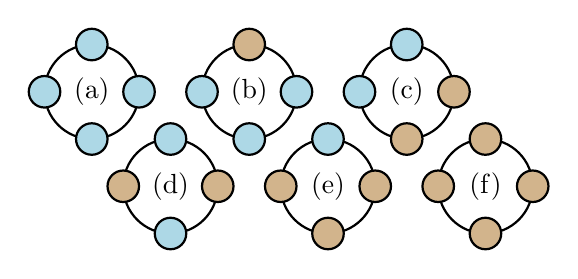
\begin{tikzpicture}
    % Define bead radius
    \def\r{0.2}
    \def\R{0.6}
    % Define colours
    \definecolor{beadblue}{RGB}{173,216,230} % Light Steel Blue
    \definecolor{beadbrown}{RGB}{210,180,140} % Tan
    
    % 1. Four blue beads
    \begin{scope}
        \draw[thick] (0,0) circle(\R);
        \foreach \i in {0,1,2,3} {
            \fill[beadblue] ({90 + 360/4*\i}:\R) circle(\r);
            \draw[thick] ({90 + 360/4*\i}:\R) circle(\r);
        }
        \node at (0,0) {(a)};
    \end{scope}
    
    % 2. Three blue, one brown
    \begin{scope}[xshift=2cm]
        \draw[thick] (0,0) circle(\R);
        \foreach \i in {0,1,2,3} {
            \ifnum\i=0
                \fill[beadbrown] ({90 + 360/4*\i}:\R) circle(\r);
            \else
                \fill[beadblue] ({90 + 360/4*\i}:\R) circle(\r);
            \fi
            \draw[thick] ({90 + 360/4*\i}:\R) circle(\r);
        }
        \node at (0,0) {(b)};
    \end{scope}
    
    % 3. Two blue, two brown (blue adjacent)
    \begin{scope}[xshift=4cm]
        \draw[thick] (0,0) circle(\R);
        \foreach \i in {0,1,2,3} {
            \ifnum\i=0
                \fill[beadblue] ({90 + 360/4*\i}:\R) circle(\r);
            \else
                \ifnum\i=1
                    \fill[beadblue] ({90 + 360/4*\i}:\R) circle(\r);
                \else
                    \fill[beadbrown] ({90 + 360/4*\i}:\R) circle(\r);
                \fi
            \fi
            \draw[thick] ({90 + 360/4*\i}:\R) circle(\r);
        }
        \node at (0,0) {(c)};
    \end{scope}
    
    % 4. Two blue, two brown (alternating)
    \begin{scope}[xshift = 1cm, yshift=-1.2cm]
        \draw[thick] (0,0) circle(\R);
        \foreach \i in {0,1,2,3} {
            \ifnum\i=0
                \fill[beadblue] ({90 + 360/4*\i}:\R) circle(\r);
            \else
                \ifnum\i=1
                    \fill[beadbrown] ({90 + 360/4*\i}:\R) circle(\r);
                \else
                    \ifnum\i=2
                        \fill[beadblue] ({90 + 360/4*\i}:\R) circle(\r);
                    \else
                        \fill[beadbrown] ({90 + 360/4*\i}:\R) circle(\r);
                    \fi
                \fi
            \fi
            \draw[thick] ({90 + 360/4*\i}:\R) circle(\r);
        }
        \node at (0,0) {(d)};
    \end{scope}
    
    % 5. One blue, three brown
    \begin{scope}[xshift= 3cm, yshift=-1.2cm]
        \draw[thick] (0,0) circle(\R);
        \foreach \i in {0,1,2,3} {
            \ifnum\i=0
                \fill[beadblue] ({90 + 360/4*\i}:\R) circle(\r);
            \else
                \fill[beadbrown] ({90 + 360/4*\i}:\R) circle(\r);
            \fi
            \draw[thick] ({90 + 360/4*\i}:\R) circle(\r);
        }
        \node at (0,0) {(e)};
    \end{scope}
    
    % 6. Four brown beads
    \begin{scope}[xshift=5cm, yshift=-1.2cm]
        \draw[thick] (0,0) circle(\R);
        \foreach \i in {0,1,2,3} {
            \fill[beadbrown] ({90 + 360/4*\i}:\R) circle(\r);
            \draw[thick] ({90 + 360/4*\i}:\R) circle(\r);
        }
        \node at (0,0) {(f)};
    \end{scope}
    
    \end{tikzpicture}
    \caption{The six binary necklaces of length $4$.}
    \label{fig:3}
    \end{figure}
    
    To determine the cycle indicators of the powers $r^m$, for $1\leq m \leq n$, we start with any element $i \in \llbracket n \rrbracket$ and repeatedly apply $r^m$ until we return to $i$. The number of applications before the first return to $i$ is the smallest positive integer $a$ such that $i + am \equiv i \mod{n}$, which simplifies to $am \equiv 0 \mod{n}$. Thus $a = n/\gcd(m,n)$, and $r^m$ is made up of $\gcd(m,n)$ cycles of length $a = n/\gcd(m,n)$, meaning its cycle indicator is $z_{n/ \gcd(m,n)}^{\gcd(m,n)}$. \smallskip
    
    To gain a more concise expression for $Z_{C_n}$, we count the number of solutions to $d=\gcd(m,n), \; 1\leq m\leq n$, for a fixed divisor $d\mid n$. This is equivalent to $\gcd(m/d ,  n/d) =1, \; 1\leq m/d  \leq n/d$, which has $\varphi(n/d)$ solutions by the definition of Euler's totient function. Hence, the cycle indicator of $Z_{C_n}$ is given by  \[Z_{C_{n}}(z_{1}, z_2, \dots, z_{n})= \frac{1}{n} \sum_{d\mid n} \varphi (n\text{/}d) z^{d}_{n\text{/}d} =\frac{1}{n} \sum_{d\mid n} \varphi (d) z^{n\text{/}d}_{d}. \]
    
    Pólya's theorem (substituting $c_j=1$ in \eqref{eq: Polya_s_theorem}) gives \begin{align*}
        N_k(n) = Z_{C_n}(k, k, \dots, k) = \frac{1}{n} \sum_{d \mid n} \varphi(n/d) k^{d}. 
    \end{align*} 
    For example, once again, 
    \[ N_2(4) = \frac{1}{4}( 2\cdot 2^1 + 1 \cdot 2^2 +  1 \cdot 2^{4} )  = 6.  \]
    
    \subsection{Dihedral Groups} What if we allow both reflections and rotations of the necklace? The relevant group becomes the dihedral group $D_{2n}$, which consists of all symmetries of a regular $n$-gon. This is the group generated by: $r$, a rotation by $2\pi/n$, as before; and $s$, a reflection across a line of symmetry of the $n$-gon. The inequivalent colourings are now called the \textit{\(k\)-ary bracelets of length $n$} and their number is denoted \(B_k(n)\) (OEIS \href{https://oeis.org/A000029}{A000029}).   \smallskip
    
    The rotations $r^m$ have the same cycle indicators as earlier, while the reflections $r^m s$ behave differently depending on whether $n$ is even or odd:

    \begin{itemize}
        \item If $n$ is odd, each reflection fixes one vertex and swaps the remaining $(n-1)/2$ pairs, so its cycle indicator is given by $z_1 z_2^{(n-1)/2}$.

        \item If $n$ is even, then half of the reflections swap $n/2$ pairs, giving a cycle indicator of $ z_2^{n/2}$. The other half fixes two opposite vertices and swaps the remaining $(n-2)/2$ pairs, giving a cycle indicator of $z_1^2 z_2^{(n-2)/2}$.
    \end{itemize} These yield that the cycle indicator of $D_{2n}$ is given by
    $$Z_{D_{2n}}(z_1, z_2,  \dots, z_n) = \begin{cases}
    \frac{1}{2 n}\left(n z_1 z_2^{(n-1) / 2}+\sum_{d \mid n} \varphi(d) z_d^{z / d}\right),&\text{if $n$ is odd,} \\
    \frac{1}{2 n}\left(\frac{n}{2} z_1^2 z_2^{(n-2) / 2}+\frac{n}{2} z_2^{n / 2}+\sum_{d \mid n} \varphi(d) z_d^{n / d}\right),&\text{if $n$ is even}.
    \end{cases}$$ Finally, Pólya's theorem yields that $B_k(n) = Z_{D_{2n}}(k, k , \dots, k)$. 

    \subsection{Symmetric Groups} Let $\mathfrak{S}_n$ denote the symmetric group of degree $n$, consisting of all permutations of the set \(\llbracket n \rrbracket\).\footnote{For clarity, the symbol $\mathfrak{S}$ denotes a calligraphic $S$.} In this subsection, rather than using $Z_{\mathfrak{S}_n}$ to obtain the generating function of the numbers of inequivalent colourings, we will do the reverse.
    
    \subsubsection{Theorem} \label{sym_group_theorem} We have \begin{equation}
    \label{eq: sym_group_thm}
    \sum_{n \geq 0 } Z_{\mathfrak
    {S}_{n}}(z_{1},z_{2},\dots,z_{n})x^{n}= \exp\left( xz_{1}+ \frac{x^{2}}{2} z_{2} + \frac{x^{3}}{3}z_{3} +\cdots \right) .
    \end{equation}  

    \begin{proof} Since $\mathfrak{S}_n$ acts transitively on each $S_{i_{1}, i_{2}, \dots}$ (that is, if two colourings of $\llbracket n \rrbracket$ use each colour the same number of times, then clearly some permutation of $\llbracket n \rrbracket$ sends one colouring to the other), it follows that $\# (S_{i_{1}, i_{2}, \dots}/\mathfrak{S}_{n})=1$ meaning that the generating function of the numbers of inequivalent colourings is given by 
    \begin{equation}
    \sum_{i_1 + i_2 + \cdots = n } \# (S_{i_{1}, i_{2}, \dots}/\mathfrak
    {S}_{n})  c_{1}^{i_{1}}c_{2}^{i_{2}} \cdots   =  \sum_{i_{1}+i_{2}+\dots =n} c_{1}^{i_{1}} c_{2}^{i_{2}} \dots . \label{eq: sym_1} 
    \end{equation} 
    
    Observe that 
    \begin{equation}
        \sum_{n \geq 0}  \left( \sum_{i_{1}+i_{2}+\dots =n} c_{1}^{i_{1}} c_{2}^{i_{2}} \dots  \right)  x^n = \frac{1}{(1-c_{1}x)(1-c_{2}x)\cdots} \label{eq: foetus_sym_group_theorem}
    \end{equation} 
    since the right-hand side expression equals $\prod_{c_j\in C}(1+c_{j}x+c_{j}^2x^2+\cdots)$ and the coefficient of $x^n$ in its expansion is the sum of all monomials of degree $n$. Moreover, by Pólya’s theorem, we can rewrite \eqref{eq: foetus_sym_group_theorem} as
    \begin{equation}
        \sum_{n \geq 0} Z_{\mathfrak{S}_n} (z_1, z_2, \dots, z_n)   x^n = \frac{1}{(1-c_{1}x)(1-c_{2}x)\cdots} \label{eq: baby_sym_group_theorem}
    \end{equation} 
    where $z_i = \sum_{c_j \in C} c_j^i$ are power sums. \smallskip
    
    To express the right-hand side in terms of the power sums, we take its logarithm, which transforms the product to a sum. Using the identities $\prod a_j = \exp (\sum \ln a_j)$ and $\ln\left( {1}/(1-x) \right)=x+\frac{x^2}{2}+\frac{x^3}{3}+\cdots$, the right-hand side of \eqref{eq: baby_sym_group_theorem} becomes
    \begin{align*}
    \prod_{c_{j} \in C} \frac{1}{(1-c_{j}x)} &= \exp \left( \sum_{c_j\in C} c_j x + \frac{c_j^2 x^2}{2} + \cdots \right) \\
    &= \exp(xz_1 + \frac{x^2}{2}z^2 + \cdots) \end{align*}which completes the proof.\footnote{More conceptually, Theorem \ref{sym_group_theorem} can be seen as a consequence of the \textit{exponential formula} \cite[p.~19]{stanleyEnumerativeCombinatoricsVolume1999}.}
    \end{proof}
    
    Furthermore, by noting that 
    \begin{align*}
    \exp\left( xz_{1}+ \frac{x^{2}}{2} z_{2} + \frac{x^{3}}{3}z_{3} +\dots \right) &= \exp(xz_{1})\cdot\exp\left( \frac{x^{2}}{2} z_{2}  \right)\cdot\exp\left( \frac{x^{3}}{3}z_{3}  \right)\cdots \\
    &=\left( \sum_{i\geq 0} \frac{x^{i}z_{1}^{i}}{i!} \right) \left( \sum_{i\geq 0} \frac{x^{2i}z_{2}^{i}}{2^{i}i!} \right) \left( \sum_{i\geq 0} \frac{x^{3i}z_{3}^{i}}{3^{i}i!} \right) \cdots,
    \end{align*}
    and comparing the coefficients of $x^n$ in \eqref{eq: sym_group_thm}, we derive that the coefficient of $z_{1}^{i_{1}}z_{2}^{i_{2}}\cdots z_{n}^{i_{n}}$ in $n! Z_{\mathfrak{S}_{n}}(z_{1},\dots,z_{n})$ (i.e. the number of permutations in $\mathfrak{S}_{n}$ with cycle type $(i_{1},i_{2},\dots ,i_{n})$ where $i_1+2i_2 +\cdots + ni_n = n$) is equal to ${n!}/{1^{i_1}i_{1}!2^{i_{2}}i_{2}!\cdots n^{i_{n}}i_{n}!}$ -- giving a more explicit formula for the cycle indicator of $$Z_{\mathfrak{S}_{n}}(z_1, z_2, \dots) =\sum_{i_{1}+2i_{2}+\cdots + ni_{n}=n}  \frac{z_{1}^{i_{1}} z_{2}^{i_{2}}  \cdots z_{n}^{i_{n}}}{i_{1}!i_{2}!\cdots i_{n}!\cdot 1^{i_{1}} 2^{i_{2}} \cdots n^{i_{n}} } .$$ This fact has, of course, a more direct combinatorial proof (see \cite[p.~30]{stanleyEnumerativeCombinatoricsVolume1}).

    \subsubsection{Example \textnormal{(Derangements)}}There are many interesting applications of Theorem \ref{sym_group_theorem} relating to counting permutations of a given cycle type. Consider the following example. \smallskip
    
    Let $d_n$ be the number of \textit{derangements} of $n$ elements which is the number of permutations of $n$ elements with no fixed points or the number of permutations in \(\mathfrak{S}_n\) with zero cycles of length $1$ (OEIS \href{https://oeis.org/A000166}{A000166}). For example, $d_{52}/{52!}$ is the probability that no card is fixed when one shuffles a standard deck of cards, assuming each permutation is equally likely. \smallskip
    
    Since we have $$d_n = n! Z_{\mathfrak{S}_n}(z_1 = 1; z_i = 0; i\neq 1),$$ Theorem \ref{sym_group_theorem} gives 
    \begin{align*}
    \sum_{n\geq 0}  \frac{d_n}{n!}x^n &= \exp \left(\frac{x^{2}}{2}  + \frac{x^{3}}{3} +\dots \right)  = \exp(-\ln(1-x)-x) \\
    &= \frac{e^{-x}}{1-x} = \left( \sum_{i = 0}^{\infty} \frac{(-x)^i}{i!} \right)  \left( \sum_{j = 0}^{\infty} x^{j} \right).
    \end{align*}
    Comparing the coefficients of $x^n$ gives
    \begin{equation}
        d_n = n! \sum_{i = 0}^{n}  \frac{(-1)^i}{i!}\sim \frac{n!}{e}. \label{eq: derangements}
    \end{equation}
    Also, we immediately derive the following recurrence relations
    \begin{align*}
        d_n &= nd_{n-1} + (-1)^n \\
        d_n &= (n-1)(d_{n-1}+d_{n-2}).
    \end{align*} The standard combinatorial proof of \eqref{eq: derangements} uses the inclusion-exclusion principle. However, the value of this generating function approach is not that it simplifies this particular problem, but that it scales effortlessly to more complex ones (for example, how many permutations of $n$ elements have three $2$-cycles and two $3$-cycles). Moreover, generating functions offer a convenient way for computing the expectation and variance of various random permutation statistics and can be made even more convenient with the use of computer algebra. These techniques are used in the analysis of randomised algorithms.  \smallskip

    \section{De Bruijn's Generalisation}

    In this section, we generalise our setup by supposing we have not only a finite group $G$ of permutations of $D$ but another finite group $H$ of permutations of $C$. We say that two colourings $f_1, f_2 \in C^D$ are equivalent if there exist $g_1 \in G$ and $h_1 \in H$ such that 
    \begin{equation*}
        f_1 =  h(f_2(g(d))), \quad \text{for all }d\in D.
    \end{equation*}
    The quotient space of this equivalence relation can be seen equally as the orbit space of $C^D$ under the following right action of $G \times H$ \begin{equation*}
        f*(g,h) = h^{-1} \circ f \circ g, \quad (g,h)\in G\times H, \; f\in C^D.
    \end{equation*}
    Burnside's lemma tells us that the number of orbits equals the average number of fixed functions over each $(g,h) \in G\times H$. Once again, we'll see that the cycle structures of $g$ and $h$ directly influence the number of fixed colourings. 
    \subsection{Lemma} The number of orbits is given by 
    \begin{equation}\label{eq: deBruijns_lemma}
        \frac{1}{\# H} \sum_{h \in H} Z_G(p_1(h), p_2(h), \dots), 
    \end{equation}
    where \(p_i(h) = \sum_{ j \mid i} c_{j}(h),\) and $c_j(h)$ denotes the number of cycles in $h$ of length $j$. \newline

    The key idea in de Bruijn's proof \cite[Sect 5.12]{deBruijnAppliedCombinatorialMathematics} is that when a given pair \((g,h)\) is applied, the fixed functions \(f \in C^D\) are exactly those for which the colour assigned to each cycle in \(g\) is chosen from a compatible cycle in $h$  -- that is, for a cycle of length \(i\) in \(g\), its colour must be fixed by $h^i$ which is true if and only if it lies in a cycle of \(h\) whose length divides \(i\). This condition forces the total number of fixed colourings to factor as a product over lengths $i$ of the cycles in \(g\), with each factor equal to \(p_i(h)=\sum_{j\mid i} c_j(h)\), where \(c_j(h)\) is the number of cycles of length \(j\) in \(h\). Averaging over \( (g,h)\in G\times H\), as prescribed by Burnside’s lemma, gives the stated formula.\medskip

    Furthermore, de Bruijn observes that \eqref{eq: deBruijns_lemma} can be interpreted in terms of derivatives. 

    \subsection{Theorem} 
    The number of orbits is given by 
    \begin{equation*}
    Z_G\left(\frac{\partial}{\partial z_1}, \frac{\partial}{\partial z_2}, \frac{\partial}{\partial z_3},  
    \cdots \right) Z_H\left(e^{z_1+z_2+z_3+\cdots}, e^{2\left(z_2+z_4+z_6+\cdots\right)}, e^{3\left(z_3+z_6+z_9+\cdots\right)}, \ldots\right),
    \end{equation*}
    evaluated at $z_1=z_2 = z_3 = \cdots = 0$. \newline
    
    The key idea in its proof is that a power $a^b$ can be seen as the $b$th derivative of $e^{az}$ evaluated at $z=0$. The stated formula can then be seen as the result of routine algebraic manipulations (see reference for details). \smallskip

    For example \cite[Exercise~10]{stanley2013}, let $n$ be the number of two-coloured necklaces of four beads, where we may also interchange the two colours to get an equivalent colouring. Thus $Z_G=\frac{1}{4}\left(z_1^4+z_2^2+2 z_4\right)$ and $Z_H=\frac{1}{2}\left(z_1^2+z_2\right)$. Hence $$\begin{aligned}
    n & =\left.\frac{1}{4} \cdot \frac{1}{2}\left(\frac{\partial^4}{\partial z_1^4}+\frac{\partial^2}{\partial z_2^2}+2 \frac{\partial}{\partial z_4}\right)\left(e^{2\left(z_1+z_2+z_3+\cdots\right)}+e^{2\left(z_2+z_4+z_6+\cdots\right)}\right)\right|_{z_i=0} \\
    & =\left.\frac{1}{8}\left(\frac{\partial^4}{\partial z_1^4}+\frac{\partial^2}{\partial z_2^2}+2 \frac{\partial}{\partial z_4}\right)\left(\frac{\left(2 z_1\right)^4}{4!}+\frac{\left(2 z_2\right)^2}{2!}+\frac{2 z_4}{1!}+\frac{\left(2 z_2\right)^4}{4!}+\frac{2 z_4}{1!}\right)\right|_{z_i=0} \\
    & =\frac{1}{8}(16+4+4+4+4) \\
    & =4.
    \end{aligned}$$
    This corresponds to the fact that the pairs $(a), (f)$ and $(b),(e)$ are the only equivalent necklaces in Figure \ref{fig:3}. \smallskip 

    Harary and Palmer \cite[Theorem 4]{HARARY1966157} provide a formula for the generating function of the numbers of inequivalent colourings, which I will not present here for the sake of brevity. In their paper, they also present interesting applications of their formula to graphical enumeration.


    \section{Conclusion} Burnside's lemma states that the number of orbits in a set of functions under the composition action of a permutation group of the domain equals the average number of fixed points over the group elements. \smallskip
    
    Pólya's theorem builds on this by showing that the number of functions fixed by a given permutation factors as a product of over its cycles. This leads to a closed formula for the generating function of the numbers of inequivalent colourings in terms of the cycle indicator of the permutation group. Harary and Palmer extend this result to the case where we have both a finite permutation group of the domain and the codomain. Both theorems lend themselves to the enumeration, asymptotic, and general analysis of many combinatorial structures. \smallskip 

    Furthermore, in studying the cycle indicators of symmetric groups, we discover an interesting formula for their ordinary generating function involving the exponential function. Further studies (see \cite[p.~19]{stanleyEnumerativeCombinatoricsVolume1999}) provide a more conceptual understanding of this link.

    

    \section*{Acknowledgments}

    We appreciate Thomas Hudson for his helpful comments. 

    
    \bibliographystyle{plain}
    \bibliography{mybib}

    


\end{document}
